% Options for packages loaded elsewhere
\PassOptionsToPackage{unicode}{hyperref}
\PassOptionsToPackage{hyphens}{url}
\PassOptionsToPackage{dvipsnames,svgnames*,x11names*}{xcolor}
%
\documentclass[
  12pt,
]{article}
\usepackage{lmodern}
\usepackage{amssymb,amsmath}
\usepackage{ifxetex,ifluatex}
\ifnum 0\ifxetex 1\fi\ifluatex 1\fi=0 % if pdftex
  \usepackage[T1]{fontenc}
  \usepackage[utf8]{inputenc}
  \usepackage{textcomp} % provide euro and other symbols
\else % if luatex or xetex
  \usepackage{unicode-math}
  \defaultfontfeatures{Scale=MatchLowercase}
  \defaultfontfeatures[\rmfamily]{Ligatures=TeX,Scale=1}
\fi
% Use upquote if available, for straight quotes in verbatim environments
\IfFileExists{upquote.sty}{\usepackage{upquote}}{}
\IfFileExists{microtype.sty}{% use microtype if available
  \usepackage[]{microtype}
  \UseMicrotypeSet[protrusion]{basicmath} % disable protrusion for tt fonts
}{}
\makeatletter
\@ifundefined{KOMAClassName}{% if non-KOMA class
  \IfFileExists{parskip.sty}{%
    \usepackage{parskip}
  }{% else
    \setlength{\parindent}{0pt}
    \setlength{\parskip}{6pt plus 2pt minus 1pt}}
}{% if KOMA class
  \KOMAoptions{parskip=half}}
\makeatother
\usepackage{xcolor}
\IfFileExists{xurl.sty}{\usepackage{xurl}}{} % add URL line breaks if available
\IfFileExists{bookmark.sty}{\usepackage{bookmark}}{\usepackage{hyperref}}
\hypersetup{
  pdftitle={Assignment FSE},
  pdfauthor={Dorian Quelle \& Frederic Denker},
  colorlinks=true,
  linkcolor=Maroon,
  filecolor=Maroon,
  citecolor=Blue,
  urlcolor=blue,
  pdfcreator={LaTeX via pandoc}}
\urlstyle{same} % disable monospaced font for URLs
\usepackage[margin=3cm]{geometry}
\usepackage{graphicx,grffile}
\makeatletter
\def\maxwidth{\ifdim\Gin@nat@width>\linewidth\linewidth\else\Gin@nat@width\fi}
\def\maxheight{\ifdim\Gin@nat@height>\textheight\textheight\else\Gin@nat@height\fi}
\makeatother
% Scale images if necessary, so that they will not overflow the page
% margins by default, and it is still possible to overwrite the defaults
% using explicit options in \includegraphics[width, height, ...]{}
\setkeys{Gin}{width=\maxwidth,height=\maxheight,keepaspectratio}
% Set default figure placement to htbp
\makeatletter
\def\fps@figure{htbp}
\makeatother
\setlength{\emergencystretch}{3em} % prevent overfull lines
\providecommand{\tightlist}{%
  \setlength{\itemsep}{0pt}\setlength{\parskip}{0pt}}
\setcounter{secnumdepth}{-\maxdimen} % remove section numbering
\usepackage{dcolumn}
\usepackage{setspace}
\doublespacing
\usepackage[utf8]{inputenc}
\usepackage{float}
\usepackage{xcolor}
\usepackage{lipsum}

\title{Assignment FSE}
\author{Dorian Quelle \& Frederic Denker}
\date{August 05, 2020}

\begin{document}
\maketitle

\hypertarget{research-summary}{%
\subsection{Research Summary:}\label{research-summary}}

This paper attempts to uncover the drivers of the willingness to donate
through the usage of a Factorial Survey Experiment. We identified
several of biases such as mental account whose impact on the donation
willingness was assessed in this paper. However, we were not able to
identify any of these biases that had a very strong and significant
impact. We can however state with high confidence that the cause for
which people donate matters immensely. While it may be considered common
knowledge, this paper still adds to the literature by examining these
hypotheses with a new and improved method increasing the ability to
potentially make causal statements.

\hypertarget{research-question}{%
\subsection{Research Question:}\label{research-question}}

\textbf{What are the drivers of donating money to charity?}

\hypertarget{keywords}{%
\subsection{Keywords}\label{keywords}}

Factorial survey experiment, donation, nudging

\newpage

\hypertarget{introduction}{%
\subsubsection{Introduction}\label{introduction}}

Donations for humanitarian purposes are essential for many organizations
and regions of the world. There is much research in the literature to
understand why and how people donate money (Bennett 2003). Although
there are discussions about the efficiency and long-term effects of
charitable donations and foreign aid (Sachs et al. 2004), millions of
people, through no fault of their own, find themselves in situations
where donations are essential for survival. From this fact and the
mandate of the UN Universal Declaration of Human Rights (ART 1 and 3)
``All human beings are born free and equal in dignity and rights'',
``Everyone has the right to life, liberty and security of person''. it
follows that at this point it is not possible to refrain from making
donations. In this study, we will not focus on the moral and economic
implications of donations, but the literature on the positive effects is
considerate. In this paper we are interested in understanding why people
donate and what they donate for. The results of this experiment will
help charitable organizations to better adapt fundraising to their
specific circumstances. This should maximize the amount of money donated
to charity and in the long-run result in higher welfare creation in
developing nations enabled through increased donations. Summing it up
this research is aiming to further the understanding of the following
question: \textbf{What are the drivers of donating money to charity?}

\hypertarget{theory-and-methodology}{%
\subsection{Theory and Methodology}\label{theory-and-methodology}}

\hypertarget{the-factorial-survey-methodology}{%
\subsubsection{The Factorial Survey
Methodology}\label{the-factorial-survey-methodology}}

Ample research in this field is normally based on empirical analyses of
the donation behavior of specific population groups (Konrath and Handy
2018). While this approach reflects reality more accurately because it
takes a multitude of factors into account when individuals make
decisions, it is precisely here that the weakness of this analysis
technique lies. Research into donation behavior can be argued to have a
blind spot for both desirability bias / clear social norms and
endogeneity baked into many of the analyses (Grimm 2010). Although
Factorial Surveys are not a new approach in the field, there is much
potential in using them to better understand drivers of human judgment.
Traditional surveys have to deal with the problem of multicollinearity
which Factorial surveys can address through making sure that factors are
orthogonal (Rossi and Nock 1982). This method combines the advantages of
an experiment with those of a questionnaire. From surveys, Factorial
Survey Experiments (FSE) takes the higher ability to achieve
heterogeneous samples and therefore higher external validity and from
experiments the higher internal validity through randomization of the
instrument. Especially when focusing on one specific issue, Factorial
Surveys can even be used to establish within-respondent comparisons by
confronting the respondent to similar but slightly changed situations
repeatedly, something that comes closer to having a true counter-factual
than many other survey methodologies. Within-respondent comparisons will
not be utilized in this paper as it falls beyond the scope of the
research question. Summarizing, using Factorial Survey Experiments
allows a significantly easier argument for causality due to researchers
to control a much higher number of factors.

\hypertarget{theoretical-background}{%
\subsubsection{Theoretical Background}\label{theoretical-background}}

In this section, we will explain the theoretical connections of
individual variables and dimensions with the willingness to donate. The
first variable is the origin of the money that the participant should
imagine to have received. Several authors have already investigated how
different origins of money can change the probability and amount of a
donation. For example, Steinberg et al.~find in their study
``Inheritance and Charitable Donations'' that inherited money has a
significantly higher elasticity in donations than earned money. The
theoretical argumentation used by the authors is the ``Mental Accounting
Theory'' according to Shefrin and Thaler (Thaler 1999). Mental
accounting is used in behavioural economics as an approach to explain
the varying handling of different (objectively often equivalent)
financial transactions. Thaler's analyses for empirical anomalies in
orthodox economics and his analysis of mental accounting earned him a
Nobel Prize in 2017. Accordingly, his theories are widely accepted and
represent the modern basis for behavioural economics. In our study the
variable takes the values:

\begin{itemize}
\tightlist
\item
  Tax refund
\item
  Bonus
\item
  Gift from mother
\end{itemize}

The tax refund is a windfall gain where we expect the elasticity of the
donations to be relatively high. (XXX) Furthermore, the variable should
point out the positive aspects of a nation state (REVISION) and thus be
linked to the aim of the donation. The interaction with the objectives
of the donation will be examined in more detail at a later stage. The
second variable, the bonus, represents the origin ``earned money''.
Since the money itself was earned here, we assume that there will be a
significantly lower elasticity and willingness to donate (Gasiorowska et
al. 2016). Because people feel as if they have a claim to the money.
Furthermore, studies have already confirmed that people are driven into
a ``market mode'' by self-earned money. Here people become less
cooperative and less social. They live more according to the motto:
``When everyone thinks of themselves, everyone is thought of''(ebd.).
Lastly, we will focus on the expression ``gift of the mother''. A gift
from the mother is a windfall gain but is often connected with the norm
that the money is spent for the own or common good. Therefore we expect
that the willingness to donate will decrease ((Zelizer 1989)).

In summary, our hypotheses regarding the first variable are:

\begin{itemize}
\tightlist
\item
  H1a: \(\beta_{taxrefund} > 0\)
\item
  H1b: \(\beta_{earnedmodey} < 0\)
\item
  H1c: \(\beta_{giftfrommother} < 0\)
\end{itemize}

The next two variables we will consider are the income of the person and
the amount of money received by each participant. The income of a person
is a variable that in most cases correlates positively with the amount
of donations. (e.g.~CHANG, Wen-Chun. ``Determinants of donations'') The
participants in our study should imagine that they either have a ``well
paying job'' or a ``poorly paying job''. Thus, we expect that the
willingness to donate increases with rising income, i.e.~with a positive
manifestation of the binary coded variable ``well paying job''. Further,
participants should imagine that they received varying amounts of money
through the previously described channels. The values of this variable
were logarithmically increasing: 10, 100 \& 1000 €. The range of values
of the variable was determined by considering to what extent the amount
of money would be logically compatible with the channels of money
transfer. For example, a 10,000 € money gift from a mother would be an
overloading of the participants' imagination. Equally unrealistic would
be a 1 € bonus. The next variable that the participants were presented
with was the goal of the humanitarian organisation. Three different
variables were coded:

\begin{itemize}
\item
  Building State Capacity = Funding the completion of a new highway
  which will connect the two main cities in Uganda
\item
  Providing education for mothers = Funding courses for women preparing
  them for Birthgiving and Motherhood
\item
  Supporting Entrepreneurs = Funding Consulting-work for SMEs in rural
  areas
\end{itemize}

Although it can be deduced from the literature that the goals of an
organization are important determinants of the donation behavior of
individuals, this was not the decisive determinant for our choice when
coding the variables. (see Why Urban Poor Donate: A Study of Low-Income
Charitable Giving in London) Our intention in coding the goals of the
organisation was to link them to the origin of the money. Here we are
once again taking up Thaler's Mental Accounting theory. If the income
and expenses were in the same mental accounts of the participants it is
expected that they will have less resistance to donate the money because
no account will be ``empty''. If we look at Richard Thaler's most
important work on this topic from 1999, we find this phenomenon in the
first section of the first page. He explains: \emph{``A few years ago I
gave a talk to a group of executives in Switzerland. After the
conference, my wife and I spent a week visiting the area. At that time
the Swiss franc was at an all-time high relative to the US dollar, so
the usual high prices in Switzerland were astronomical. My wife and I
comforted ourselves that I had received a fee for the talk that would
easily cover the outrageous prices for hotels and meals. Had I received
the same fee a week earlier for a talk in New York though, the vacation
would have been much less enjoyable.''} In a later section, he
elaborates that it was less painful to spend money in Switzerland
because he had a Swiss lecture mental account that could not negatively
impact his overall wealth as he was just being ``filled''. We expect
that this will also be the case with the participants' donations. A gift
from one's mother and Funding courses for women preparing them for
giving birth and motherhood in Uganda will be included in one Mental
Account, as will Thaler's Swiss journey. The same is true for a bonus
resulting from ones own performance and the support of SMEs in
developing countries. Finally, a tax refund and support for Uganda's
state-building capacity should also be included in only one account.
Across all of the organizations' goals, we have kept the country target
constant for two reasons. First, Uganda is one of the poorest countries
in the world. According to the CIA World Factbook, Uganda ranks 199th in
the category GDP per Capita. While this does not necessarily say
everything about the living standards and the welfare needs of the
country's inhabitants, it is a good proxy.
(\url{https://www.cia.gov/library/publications/the-world-factbook/rankorder/2004rank.html})
The low standard of living in the country where the aid is to go is
supposed to confirm the donors' expectation that the people receiving
the money will need it. The second reason is that we want to vary as few
factors as possible between the different categories to guarantee the
greatest possible validity of our estimators. Nevertheless, we will
analyse the individual interaction effects separately to rule out the
possibility that the mental linking of the accounts may not have worked
for all examples. Furthermore, especially in the case of donations with
the goal of motherhood, we will add an interaction with the variable
gender. Our hypotheses for the variable ``Goals of Donation'' are
therefore as follows:

\begin{itemize}
\item
  H2: There will be a significant positive effect of the dummy variable
  ``Equal'' which takes the value 1 if the origin and the destination of
  the money are in the same mental account. So: \(\delta_{equal} > 0\)
\item
  H2a: \(\delta_{origin:mother} \times\) \(\delta_{goal:mother}\)
  \textgreater{} 0
\item
  H2b: \(\delta_{origin:taxrefund} \times \delta_{goal:state} > 0\)
\item
  H2c: \(\delta_{origin:bonus} \times \delta_{goal:Entrepreneur} > 0\)
\end{itemize}

The last relevant dimension is the channel of money transfer. Here we
can state that money that has not yet been booked, and ,therefore, is
not attributed to a mental account, can simply be spent. This also comes
from the ``Mental Accounting'' theory. If the participant is asked to
imagine that he has not yet received the money and is asked if he would
be willing to donate this money, he does not have to credit one of his
mental accounts. We therefore expect that the willingness to donate
money not yet received is significantly higher than the willingness to
donate money already received. This leads us to the concretization of
the last hypothesis:

\begin{itemize}
\tightlist
\item
  H3: \(\mu_{received} < \mu_{notreceived}\)
\end{itemize}

\hypertarget{survey-operationalization}{%
\subsubsection{Survey
operationalization}\label{survey-operationalization}}

To be able to test these hypotheses, we use the beforementioned method
of Factorial Survey Experiments:

The initial planning was to run this experiment as Pen-and-Paper
Personal Interviews (PAPI). Due to the Covid-19 Pandemic, this was not
feasible anymore. Therefore, we resorted to sending the PDF of the
questionnaires to the respondents and asking them to print it and send
it back.

When creating the questionnaires a sampling strategy needs to be
employed. However, our survey only has 5 dimensions with 3,3,3,2,2
levels. This means that we have a universe of 108 unique vignettes.
Including 12 vignettes for each survey we able to survey the complete
universe of vignettes in 9 surveys. We surveyed 17 individuals and each
deck at least once which should increase the validity. Additionally by
choosing 5 dimensions it was the goal to give the respondents enough
detail so the description of the scenario was understandable without
using their imagination while at the same time not overburdening the
respondents.

For each of the twelve vignettes, we presented the respondent with five
dimensions for which he or she had to respond to the question \emph{How
likely is it that you are going to donate the amount?} The following
dimensions that were explained above will be quickly summarized below to
provide a clear overview:

\begin{itemize}
\tightlist
\item
  The working situation of the person who will be asked to donate. The
  available options are a minimum wage job and a well paying job.
\item
  The amount of money you receive. It can be either 10, 100 or 1000
  Euros.
\item
  The origin of the money. The available options were tax refund, gift
  from mother or a bonus from work.
\item
  The channel of the money. This differentiates between whether you have
  yet to receive the money and can decide to redirect it to the cause or
  whether you have already received the money.
\item
  Lastly, the goal of the donation which can be building state capacity
  in Uganda, supporting small businesses and entrepreneurs in Uganda or
  provide education for young mothers in Uganda.
\end{itemize}

The respondent is then asked about their likelihood of donating using a
Likert Scale with 5 values. The extremes (-2 and 2) were labelled ``Very
unlikely'' and ``Very likely'' respectively.

Below you will find one example vignette as it was presented to the
respondents:

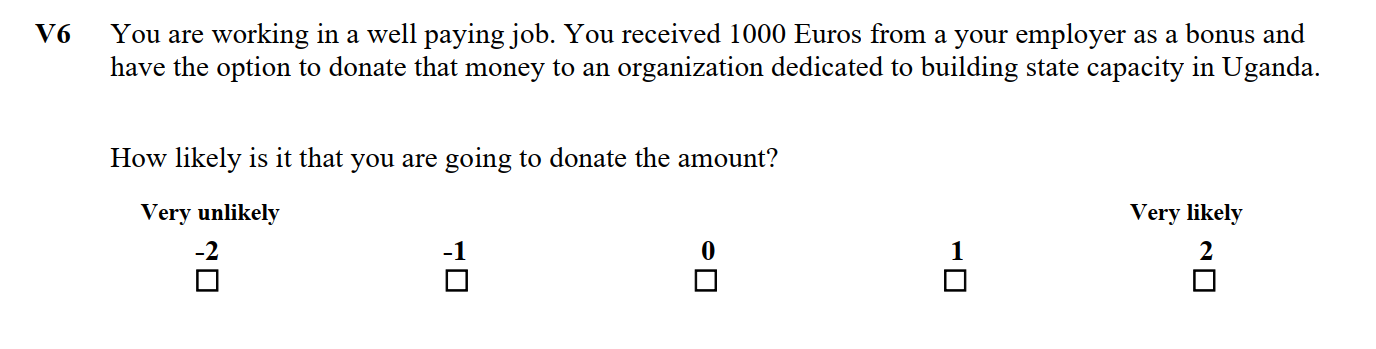
\includegraphics[width=1.05\linewidth]{Screenshot_vignette}

In addition to these 12, vignettes we asked the respondents to answer 7
questions on themselves, more specifically gender, year of birth,
country of residence and highest educational qualification were asked
before the survey. After the survey the respondents were asked how
difficult they through these imaginary descriptions were to rate, to how
many different causes they have donated in 2019 and what the approximate
amount of money they have donated in 2019. For the latter two questions
one could refuse the answer.

\hypertarget{results}{%
\subsection{Results}\label{results}}

Before looking at inferential statistics it is essential to get an
overview over the data, starting with the properties of the respondents
themselves:

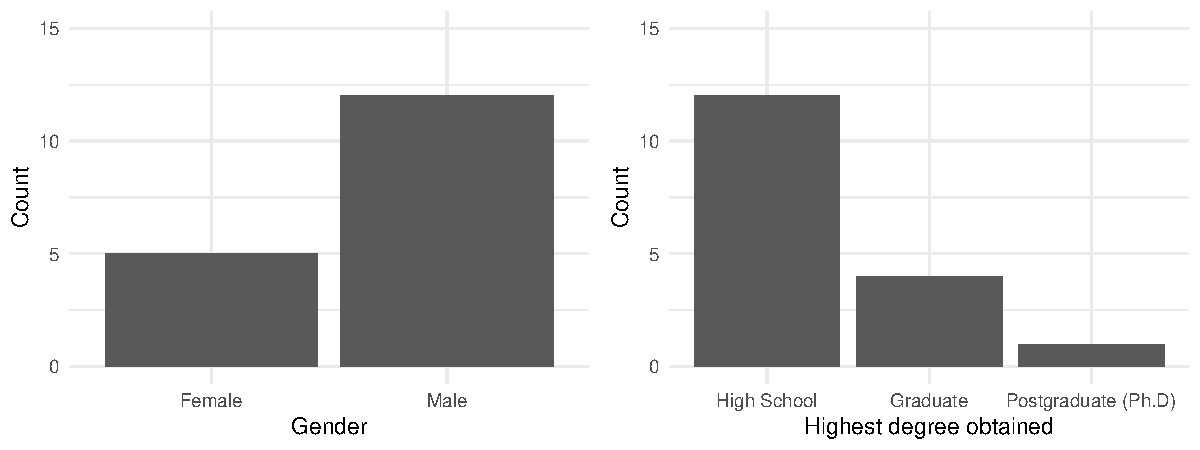
\includegraphics[width=1.05\linewidth]{FSE_paper_files/figure-latex/unnamed-chunk-2-1}

For the sake of completeness, the distribution of value for the
questions on the general difficulty of rating the situations, the number
of times donated and the total amount donated is plotted below. For the
difficulty -5 was very difficult and +5 was very easy. We can see that
for most respondents it was challenging at most which means that we
chose the number and content of the dimensions appropriately. However,
this value can be improved upon for example through an extensive
pre-test, which was out of the scope of this research endeavor.

The respondents were given the option to not give information on the
latter two questions which resulted in 1 person not giving information
of the number on times donated and three respondents for the total
amount donated.

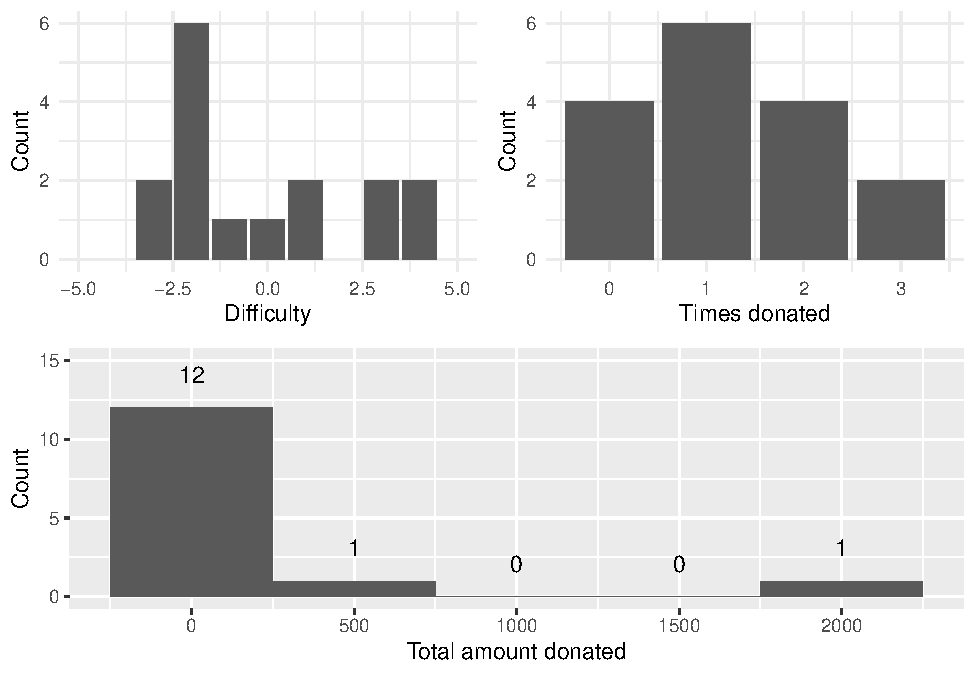
\includegraphics{FSE_paper_files/figure-latex/plotting_b_questions-1.pdf}

To give a short display of the data, the distribution of the main
outcome variable is plotted below:

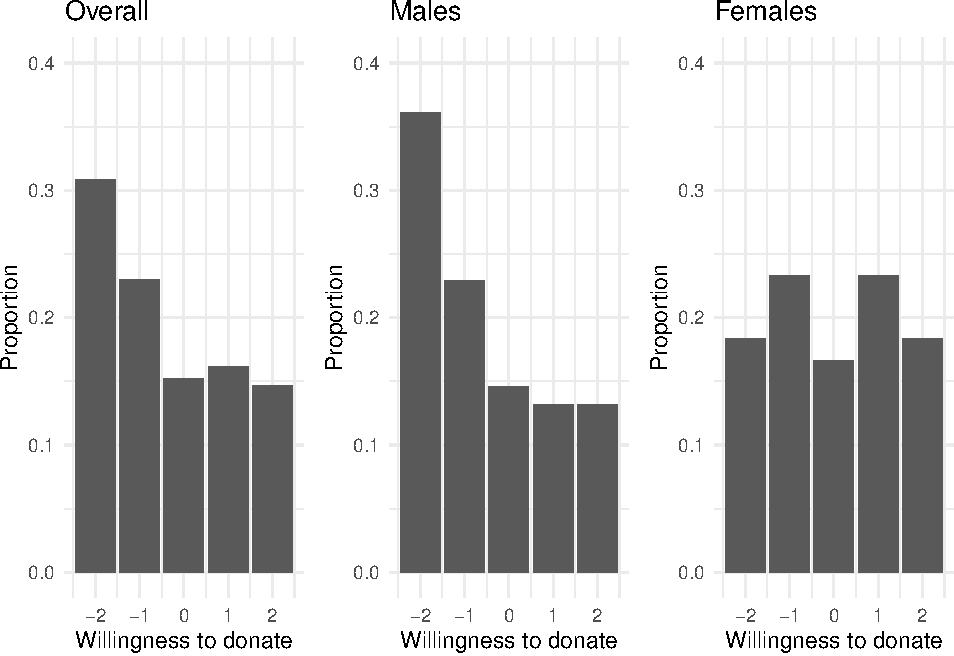
\includegraphics{FSE_paper_files/figure-latex/plotting_proportions-1.pdf}

\hypertarget{hypothesis-testing}{%
\subsubsection{Hypothesis testing}\label{hypothesis-testing}}

As informing as these descriptive plots were, we will now examine the
hypotheses one by one to assess which we can to reject. For this, we
have conducted three t-tests with \(\mu = 0\), the results of which are
displayed below:

\begin{table}[!htbp] \centering 
  \caption{T-test results | ***: p<0.01} 
  \label{} 
\begin{tabular}{@{\extracolsep{5pt}} ccccc} 
\\[-1.8ex]\hline 
\hline \\[-1.8ex] 
 & Variable & Mean & t.value & p.value \\ 
\hline \\[-1.8ex] 
1 & Tax refund & -0.576 & -3.3849 & 0.001 \textasteriskcentered \textasteriskcentered \textasteriskcentered  \\ 
2 & Bonus & -0.083 & -0.472 & 0.639 \\ 
3 & Gift from mother & -0.54 & -3.178 & 0.002 \textasteriskcentered \textasteriskcentered \textasteriskcentered  \\ 
\hline \\[-1.8ex] 
\end{tabular} 
\end{table}

\begin{table}[!htbp] \centering 
  \caption{} 
  \label{} 
\begin{tabular}{@{\extracolsep{5pt}} cccccc} 
\\[-1.8ex]\hline 
\hline \\[-1.8ex] 
 & Variable & Mean.of.x & Mean.of.y & t.value & p.value \\ 
\hline \\[-1.8ex] 
1 & Channel & -0.472 & 0.324 & -0.36747 & 0.713 \\ 
2 & Income & 0.230 & -1.04 & 7.0424 & 0.000 \\ 
\hline \\[-1.8ex] 
\end{tabular} 
\end{table}

Starting with the first hypothesis which states that
\(\beta_{taxrefund} > 0\) we can reject the hypothesis. For the
hypothesis \(H1b\) (\(\beta_{earnedmoney} < 0\)) we cannot reject the
\(H_0\) which would state that \(\beta_{earnedmoney} > 0\), so we must
also reject the \(H1b\).

We can, however, reject the Null-hypothesis for the \(H1c\) which means
that our data validate that \(\beta_{giftfrommother} < 0\), as the
theory predicts.

For the next hypotheses, we run four regression with robust standard
errors clustered on the respondents displayed below:

\begin{table}[h!] \centering 
  \caption{Regression Results with Clustered Standard Errors} 
  \label{} 
\begin{tabular}{@{\extracolsep{0.5 pt}}lD{.}{.}{-3} D{.}{.}{-3} D{.}{.}{-3} D{.}{.}{-3} } 
\\[-1.8ex]\hline 
\hline \\[-1.8ex] 
 & \multicolumn{4}{c}{\textit{Dependent variable:}} \\ 
\cline{2-5} 
\\[-1.8ex] & \multicolumn{4}{c}{Willingness to donate} \\ 
\\[-1.8ex] & \multicolumn{1}{c}{(1)} & \multicolumn{1}{c}{(2)} & \multicolumn{1}{c}{(3)} & \multicolumn{1}{c}{(4)}\\ 
\hline \\[-1.8ex] 
 Equal & -0.076 &  &  &  \\ 
  & (0.213) &  &  &  \\ 
  Origin: Gift from Mother &  & -0.362 &  &  \\ 
  &  & (0.298) &  &  \\ 
  Goal: Mothers &  & 0.913^{***} &  &  \\ 
  &  & (0.314) &  &  \\ 
  Interaction effect: Mother &  & 0.352 &  &  \\ 
  &  & (0.494) &  &  \\ 
  Origin: Tax refund &  &  & -0.084 &  \\ 
  &  &  & (0.260) &  \\ 
  Goal: State capacity &  &  & -0.618^{**} &  \\ 
  &  &  & (0.301) &  \\ 
  Interaction effect: State &  &  & -0.493^{*} &  \\ 
  &  &  & (0.292) &  \\ 
  Origin: Bonus &  &  &  & 0.573^{**} \\ 
  &  &  &  & (0.253) \\ 
  Goal: Entrepreneurship &  &  &  & -0.343^{*} \\ 
  &  &  &  & (0.177) \\ 
  Interaction effect: Individual &  &  &  & -0.152 \\ 
  &  &  &  & (0.395) \\ 
  Constant & -0.364^{*} & -0.663^{***} & -0.139 & -0.457^{**} \\ 
  & (0.219) & (0.211) & (0.206) & (0.212) \\ 
 \hline \\[-1.8ex] 
\hline 
\hline \\[-1.8ex] 
\textit{Note:}  & \multicolumn{4}{r}{$^{*}$p$<$0.1; $^{**}$p$<$0.05; $^{***}$p$<$0.01} \\ 
\end{tabular} 
\end{table}

Interestingly, these regressions do not confirm the mental accounting
theory as we are not able to reject any \(H_0\) for any of the four
hypotheses at the 5 \% significance level. For \(H1c\) we could reject
the \(H_0\) at the 10 \% significance level, however this is not the
significance level we set as we do not want to invoke any Type I errors.
While it is unfortunate for this specific paper that we could not reject
any of these hypotheses at the previously set 5 \% significance level,
it became clear for researchers in many fields that unreported null
results are a major problem (Rosenthal 1979), which is why we report
them here.

Lastly, we want to test hypothesis H3. For this we again run a
regression with robust clustered standard errors on the respondents:

\begin{table}[h!] \centering 
  \caption{Regression Results with Clustered Standard Errors} 
  \label{} 
\begin{tabular}{@{\extracolsep{0.5 pt}}lD{.}{.}{-3} } 
\\[-1.8ex]\hline 
\hline \\[-1.8ex] 
 & \multicolumn{1}{c}{\textit{Dependent variable:}} \\ 
\cline{2-2} 
\\[-1.8ex] & \multicolumn{1}{c}{Willingness to donate} \\ 
\hline \\[-1.8ex] 
 Not received  & -0.074 \\ 
  & (0.166) \\ 
  Constant (Received) & -0.356^{*} \\ 
  & (0.199) \\ 
 \hline \\[-1.8ex] 
\hline 
\hline \\[-1.8ex] 
\textit{Note:}  & \multicolumn{1}{r}{$^{*}$p$<$0.1; $^{**}$p$<$0.05; $^{***}$p$<$0.01} \\ 
\end{tabular} 
\end{table}

We cannot reject the \(H_0\) of the H3 as not receiving the money and
therefore directly donating it is not statistically significant at any
relevant significance level.

\hypertarget{discussion-and-limitations}{%
\subsection{Discussion and
Limitations}\label{discussion-and-limitations}}

This paper was able to show the benefits of Factorial Survey Experiments
in theory-led validation of common hypotheses. In this case only one
hypothesis could be confirmed/ one \(H_0\) could be rejected: We can be
fairly certain that received money with the goal of investing in mothers
education are more likely to be donated.

There are a number of limitations to this study. Firstly, is of course
the sample size which is relatively low with only 17 respondents.
However, due to the high number of vignettes that each answered (12 to
be precise) we still have a fairly high n in the end (204). It is import
to mention that the respondents were mostly male and relatively young
which might introduce a selection bias.

Furthermore, as usual in research on donations, desirability bias can
pose a challenge that this research approach tries to address by
exposing the respondent to theoretical situations under anonymity. This
should counteract the desirability bias partly, but this cannot be
proven in this context.

Another limitation of survey design lies in the sampling. We could have
increased the balance of the asked dimensions slightly by having one
more person answer the second deck which would have meant a perfect
double usage of the universe of vignettes.

\hypertarget{bibliography}{%
\subsection*{Bibliography}\label{bibliography}}
\addcontentsline{toc}{subsection}{Bibliography}

\hypertarget{refs}{}
\leavevmode\hypertarget{ref-bennettFactorsUnderlyingInclination2003}{}%
Bennett, Roger. 2003. ``Factors Underlying the Inclination to Donate to
Particular Types of Charity.'' \emph{International Journal of Nonprofit
and Voluntary Sector Marketing} 8 (1): 12--29.
\url{https://doi.org/10.1002/nvsm.198}.

\leavevmode\hypertarget{ref-gasiorowskaMoneyCuesIncrease2016}{}%
Gasiorowska, Agata, Lan Nguyen Chaplin, Tomasz Zaleskiewicz, Sandra
Wygrab, and Kathleen D. Vohs. 2016. ``Money Cues Increase Agency and
Decrease Prosociality Among Children: Early Signs of Market-Mode
Behaviors.'' \emph{Psychological Science} 27 (3): 331--44.
\url{https://doi.org/10.1177/0956797615620378}.

\leavevmode\hypertarget{ref-grimmSocialDesirabilityBias2010}{}%
Grimm, Pamela. 2010. ``Social Desirability Bias.'' In \emph{Wiley
International Encyclopedia of Marketing}, edited by Jagdish Sheth and
Naresh Malhotra, wiem02057. Chichester, UK: John Wiley \& Sons, Ltd.
\url{https://doi.org/10.1002/9781444316568.wiem02057}.

\leavevmode\hypertarget{ref-konrathDevelopmentValidationMotives2018}{}%
Konrath, Sara, and Femida Handy. 2018. ``The Development and Validation
of the Motives to Donate Scale.'' \emph{Nonprofit and Voluntary Sector
Quarterly} 47 (2): 347--75.
\url{https://doi.org/10.1177/0899764017744894}.

\leavevmode\hypertarget{ref-rosenthalFileDrawerProblem1979}{}%
Rosenthal, Robert. 1979. ``The File Drawer Problem and Tolerance for
Null Results.'' \emph{Psychological Bulletin} 86 (3): 638--41.
\url{https://doi.org/10.1037/0033-2909.86.3.638}.

\leavevmode\hypertarget{ref-rossiMeasuringSocialJudgments1982}{}%
Rossi, Peter H., and Steven L. Nock, eds. 1982. \emph{Measuring Social
Judgments: The Factorial Survey Approach}. Beverly Hills: Sage
Publications.

\leavevmode\hypertarget{ref-sachsEndingAfricaPoverty2004}{}%
Sachs, Jeffrey, John W. McArthur, Guido Schmidt-Traub, Margaret Kruk,
Chandrika Bahadur, Michael Faye, and Gordon McCord. 2004. ``Ending
Africa's Poverty Trap.'' \emph{Brookings Papers on Economic Activity}
2004 (1): 117--240. \url{https://doi.org/10.1353/eca.2004.0018}.

\leavevmode\hypertarget{ref-thalerMentalAccountingMatters1999}{}%
Thaler, Richard H. 1999. ``Mental Accounting Matters.'' \emph{Journal of
Behavioral Decision Making} 12 (3): 183--206.
\url{https://doi.org/10.1002/(SICI)1099-0771(199909)12:3\%3C183::AID-BDM318\%3E3.0.CO;2-F}.

\leavevmode\hypertarget{ref-zelizerSocialMeaningMoney1989}{}%
Zelizer, Viviana A. 1989. ``The Social Meaning of Money: "Special
Monies".'' \emph{American Journal of Sociology} 95 (2): 342--77.
\url{https://doi.org/10.1086/229272}.

\end{document}
